\section*{MAIN FIGURE TITLES AND LEGENDS}

%%% Figure 1: E/I Module Mechanism (fig1.jpg)
\begin{figure}[htbp]
\centering
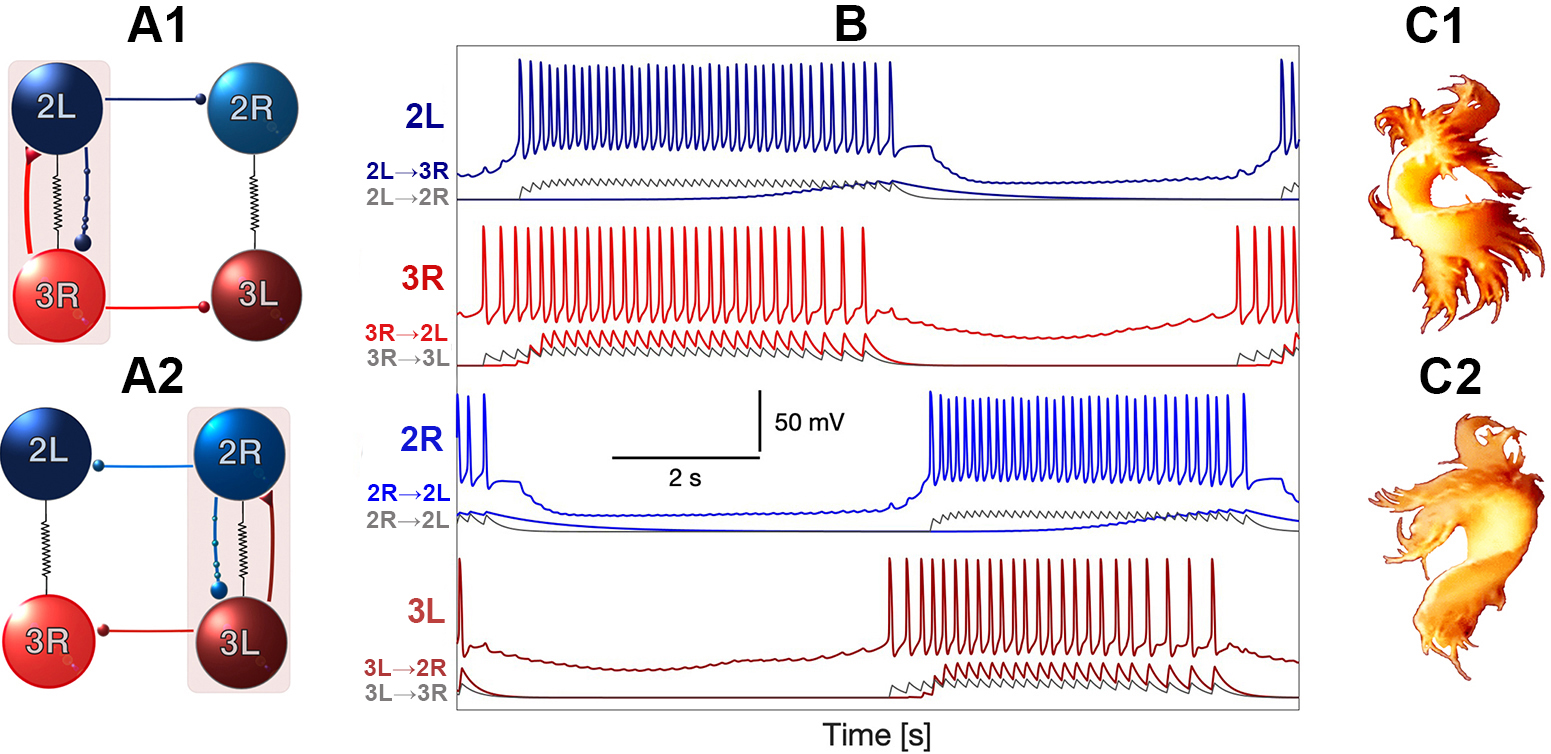
\includegraphics[width=\textwidth]{fig1.jpg}
\caption{{\bf Mechanism of left--right alternation: two reciprocally inhibitory E/I sub-networks generate anti-phase bursting.}
(A1--A2) Schematic of the contralateral E/I modules (Si3R$\leftrightarrows$Si2L and Si3L$\leftrightarrows$Si2R) embedded within reciprocally inhibitory half-center oscillators (Si3R$\leftrightarrows$Si3L below and Si2R$\leftrightarrows$Si2L above) that enforce bilateral alternation.
In A1 the right module (Si3R$\to$Si2L) is active while the left module is suppressed; in A2 the roles are reversed.
When isolated, each E/I module is tuned to be ``almost-oscillatory''---exhibiting damped oscillations or subthreshold rhythmic fluctuations rather than sustained limit cycles---so that network coupling is required to recruit them into coordinated bursting.
(B) Corresponding model voltage traces (thick colored) and simulated neurotransmitter release probabilities (thin curves): the top two traces show Si2L and Si2R, while the bottom two traces show Si3L and Si3R.
Red denotes excitatory Si3$\to$Si2 logistic synapses with faster kinetics, grey reciprocal inhibitory $\alpha$-synapses within the Si3 and within the Si2 pairs, and blue the slower logistic Si2$\to$Si3 inhibition that terminates each burst and sets episode duration.
(C1--C2) Sketch of corresponding whole-body undulations for consecutive left--right episodes.}
\label{fig:ei_mechanism}
\end{figure}

%%% Figure 2: Synaptic timescales (fig2.jpg)
\begin{figure}[htbp]
\centering

\includegraphics[width=\textwidth]{fig2.jpg}
\caption{{\bf Synaptic timescales in the model match experimental recordings.}
Compare panels~C and~D with the corresponding neurophysiological recordings presented in Fig.~7 of Sakurai \& Katz (2022).
(A--B) Three positive current pulses of progressively increasing amplitude applied to Si2R produce graded inhibitory postsynaptic potential (IPSP) responses in the contralateral Si2L, demonstrating the amplitude scaling of reciprocal inhibition.
(C--D) Two current pulses injected into Si2R evoke accumulating IPSP responses in Si2L and elicit dual-timescale responses in Si3L: a fast depolarizing component mediated by electrical coupling, followed by slower inhibition mediated by the logistic synapse.
The temporal separation between these components---tens of milliseconds for electrical coupling versus hundreds of milliseconds for chemical inhibition---matches the experimentally observed dynamics and establishes the timescales that govern burst shaping.}
\label{fig:synaptic_timescales}
\end{figure}

%%% Figure 3: CPG Assembly (fig3.jpg)
\begin{figure}[htbp]
\centering
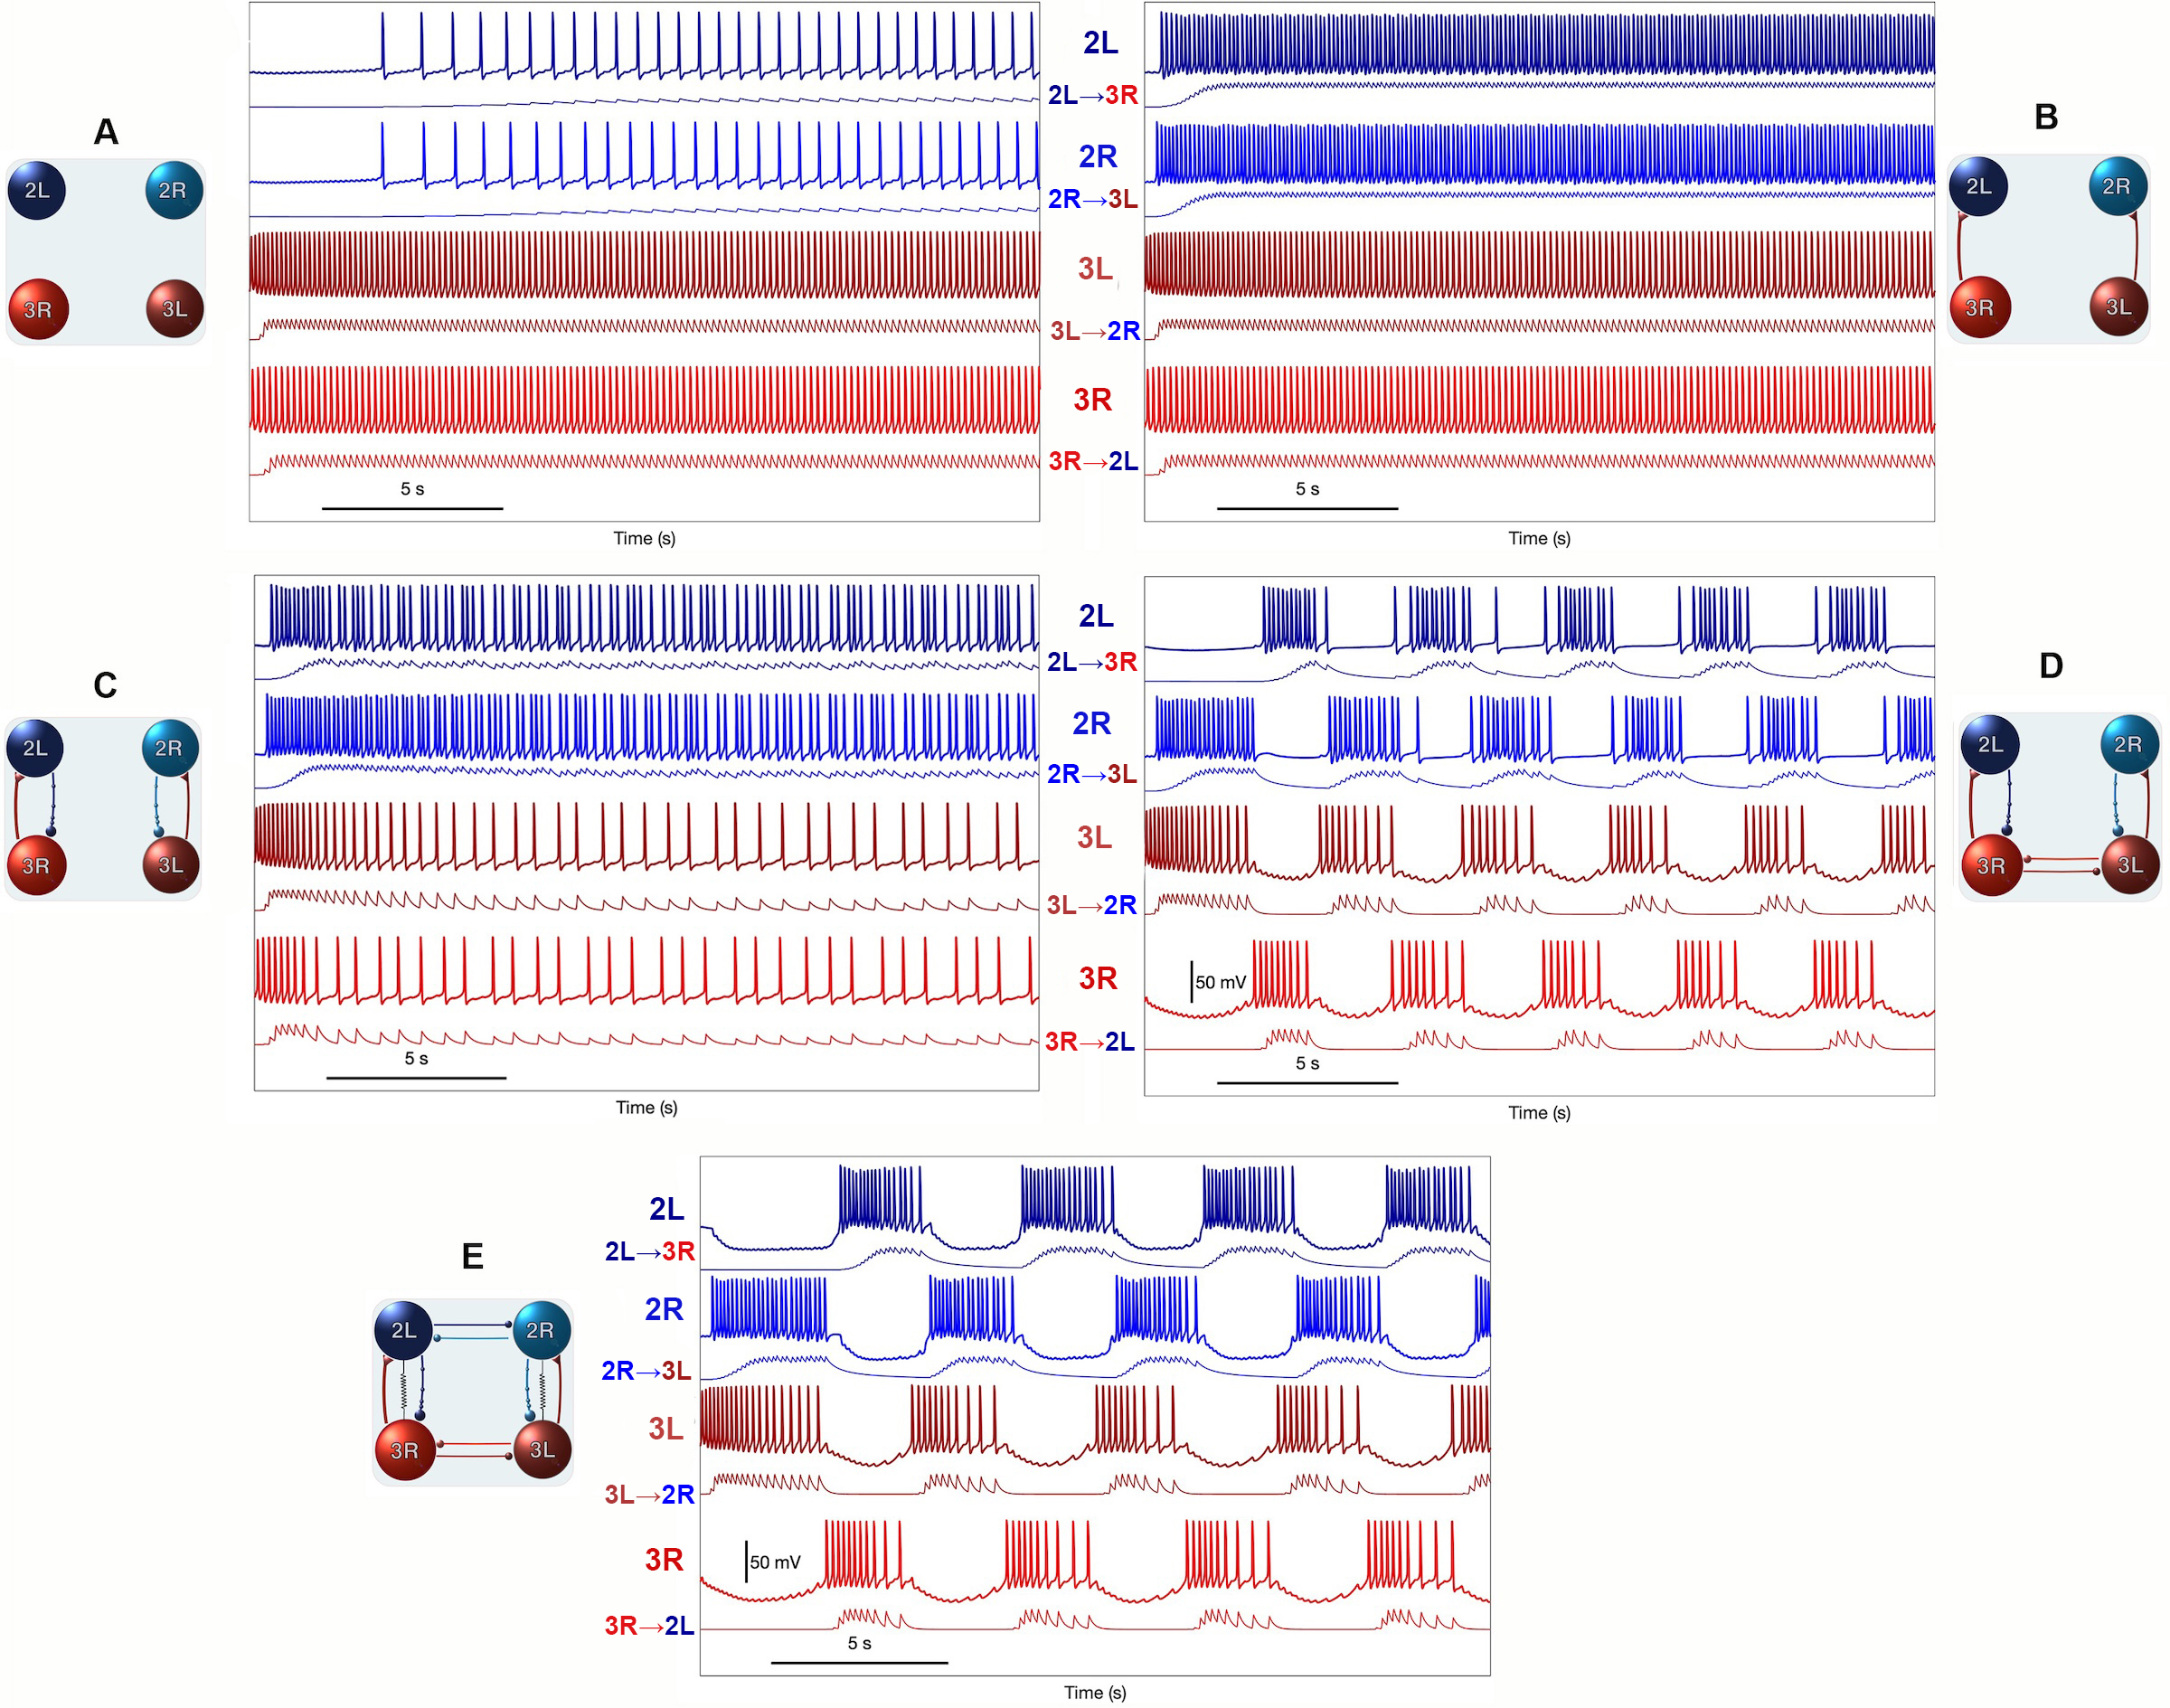
\includegraphics[width=\textwidth]{fig3.jpg}
\caption{{\bf CPG assembly in five sequential steps.}
(A) Four uncoupled interneurons, with Si3 neurons exhibiting intrinsic excitability and firing at a higher rate.
(B) Si3 neurons provide fast excitatory drive to contralateral Si2 neurons.
(C) Si2 neurons deliver slow inhibitory feedback to Si3 neurons to slow them down.
(D) Reciprocal inhibition between contralateral Si3 neurons triggers an initial rhythm formation.
(E) Reciprocally inhibitory synapses activated between contralateral Si2 neurons, along with two electrical synapses between Si3R$\leftrightarrows$Si2L and Si3L$\leftrightarrows$Si2R pairs of interneurons, generate stably the network-level bursting in the swim CPG model of \textit{Dendronotus iris}.
The traces underneath the voltage waveforms represent the corresponding neurotransmitter probability $s(t)$ in the pre-synaptic neurons.}
\label{fig:assembly}
\end{figure}

%%% Figure 4: Model vs experimental comparison (fig4.jpg)
\begin{figure}[htbp]
\centering

\includegraphics[width=\textwidth]{fig4.jpg}
\caption{{\bf Model responses to targeted perturbations match experimental recordings.}
Each panel shows model traces (top) alongside corresponding experimental recordings from Sakurai \& Katz (2016) (bottom).
(A) Depolarization of Si2L: injecting positive current into Si2L disrupts the ongoing rhythm; upon current removal, the network rapidly recovers coordinated bursting.
(B) Hyperpolarization of Si2L: injecting negative current into Si2L silences this neuron while the contralateral neurons continue oscillating; the network resumes normal activity upon release.}
\label{fig:perturbation_responses}
\end{figure}

%%% Figure 5: Si1 control and neuromodulation (fig5.jpg)
\begin{figure}[htbp]
\centering
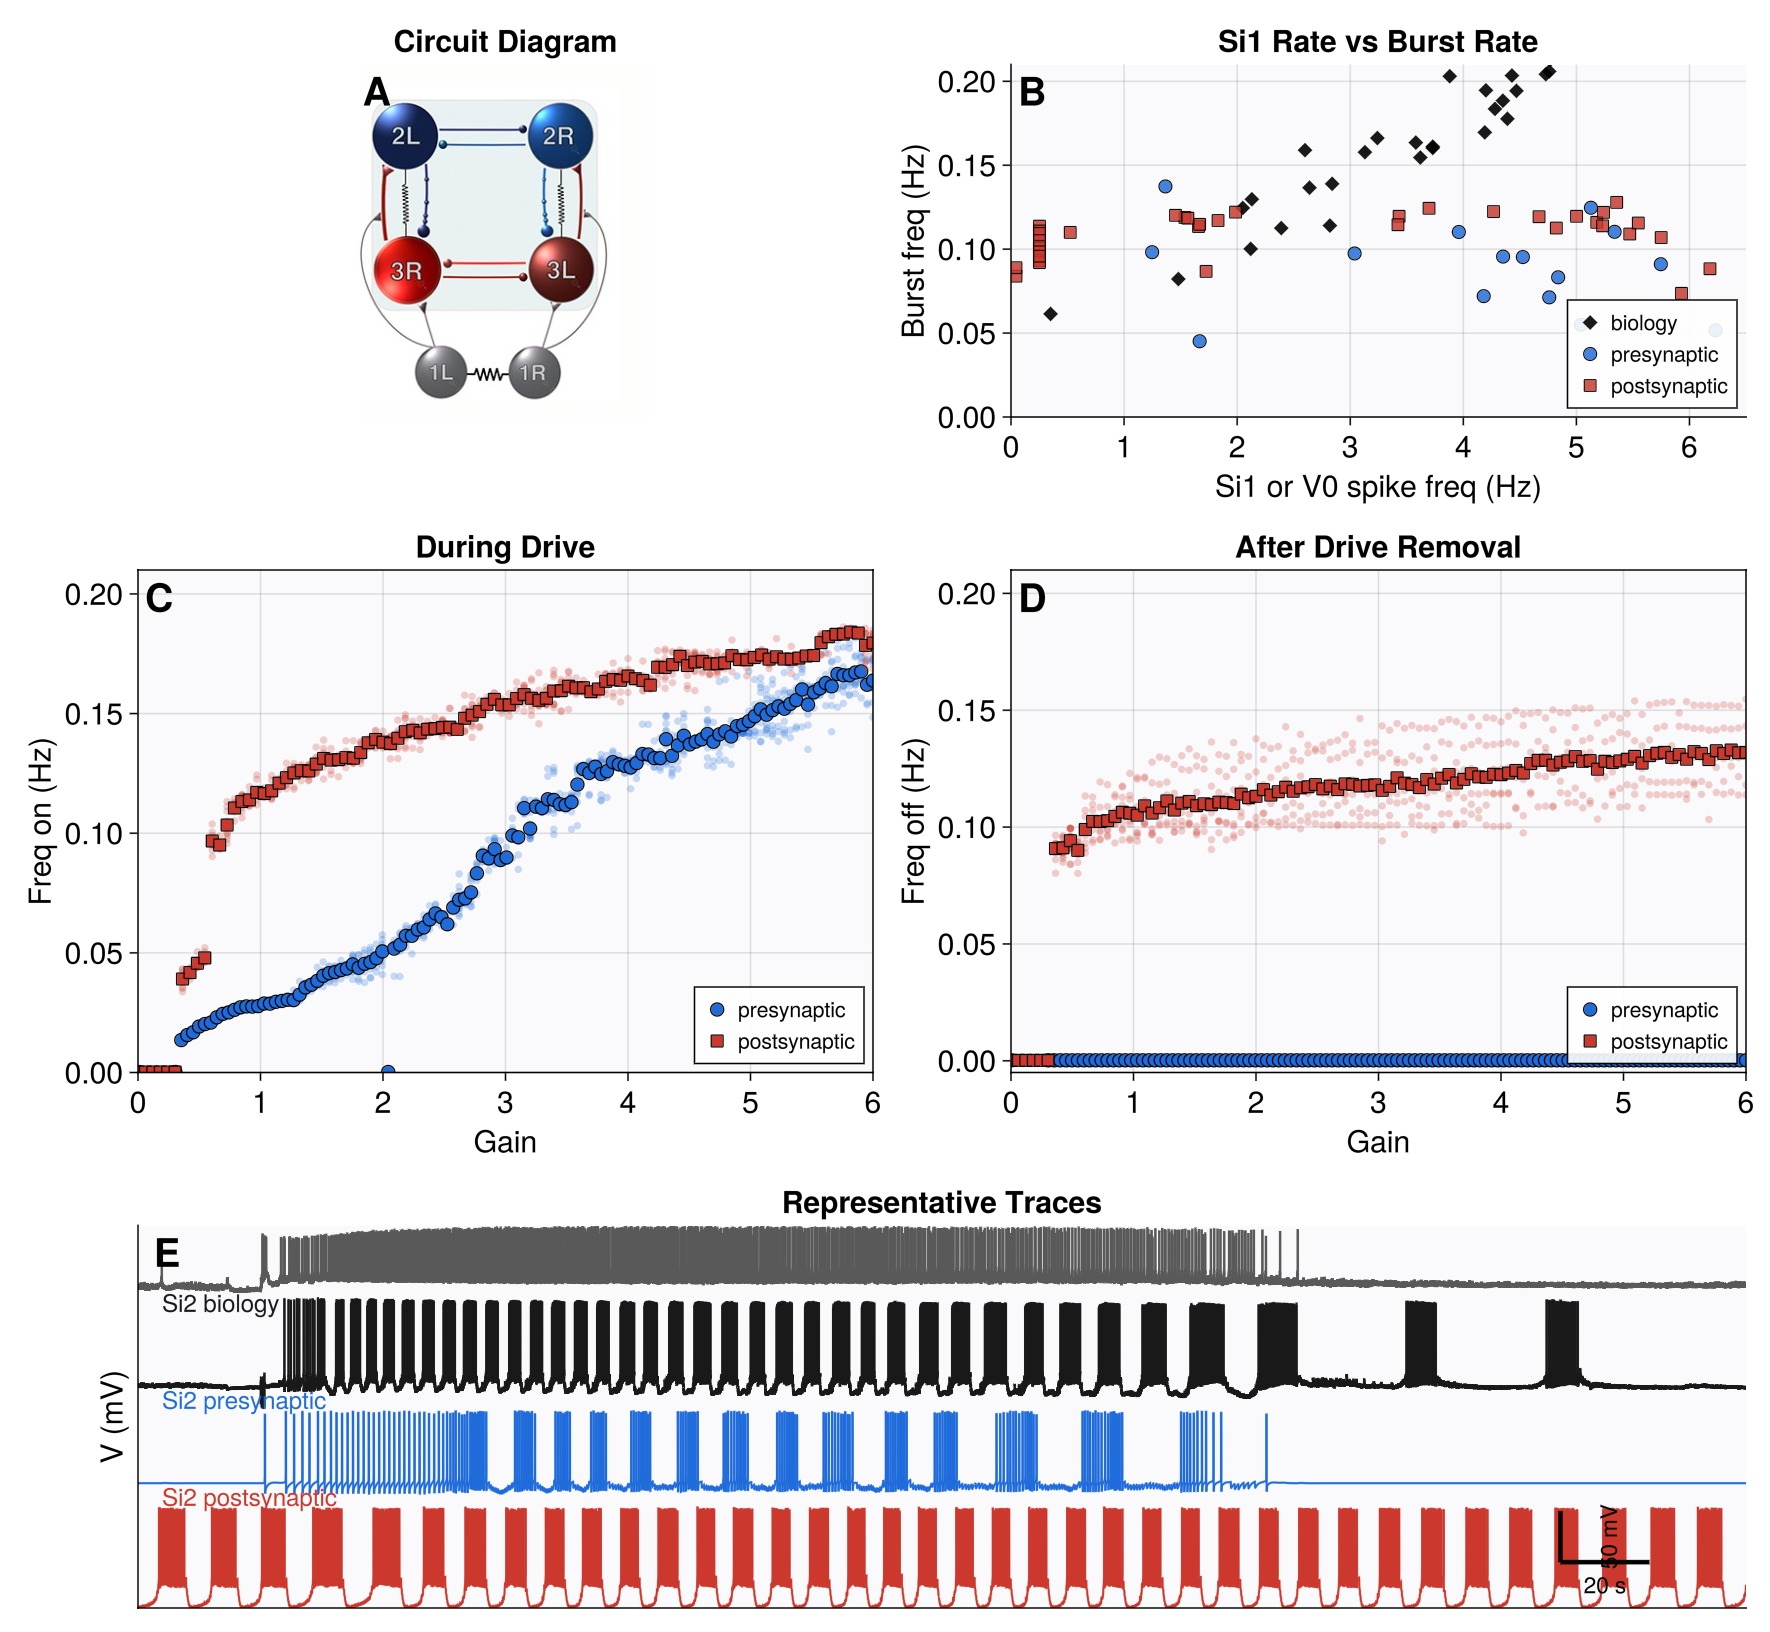
\includegraphics[width=\textwidth]{fig5.jpg}
\caption{{\bf Si1-dependent modulation of the Si3$\to$Si2 pathway regulates burst frequency during sustained drive.}
(A) Schematic of the five-cell swim circuit highlighting direct Si1 excitation of Si3 neurons and activity-dependent modulation of the Si3$\to$Si2 excitatory pathway.
(B) Relationship between Si1 spike rate and burst frequency.
Grey circles and grey fit line show digitized points from the published biological summary in Sakurai \& Katz (2019) \cite{sakurai2019command}, black triangles and black fit line show measurements extracted directly from the representative biological Si1/Si2 trace pair, and blue circles and red squares show matched model measurements from representative presynaptic and postsynaptic simulations, respectively.
(C) Scan of the dimensionless modulatory gain parameter $g_m$ during sustained drive.
In the presynaptic condition, gain multiplies the logistic Si3$\to$Si2 accumulation-rate parameter $\alpha$; in the postsynaptic condition, the same gain multiplies the effective synaptic conductance.
Both scans show gain-dependent changes in burst frequency, with different response curves for the two modulation targets.
Faint points show individual measured intervals; saturated markers show gain-wise means.
(D) Representative biological and model traces.
Top two traces show the biological Si1 and Si2 recordings.
Blue and red traces show the corresponding Si2 activity produced by presynaptic and postsynaptic model variants under the same Si1 drive, and the purple trace shows the shared modulatory variable $s_m$.
Triangles, circles, and squares mark detected burst onsets from the biological, presynaptic, and postsynaptic traces, respectively, and these onset-to-onset intervals are the measurements used for the rate-matching analysis in panel B.
The scale bar in panel D denotes 20~s and 50~mV.}
\label{fig:si1_neuromod}
\end{figure}

%%% Figure 6: Summary / Conclusion (fig6.jpg)
\begin{figure}[htbp]
\centering
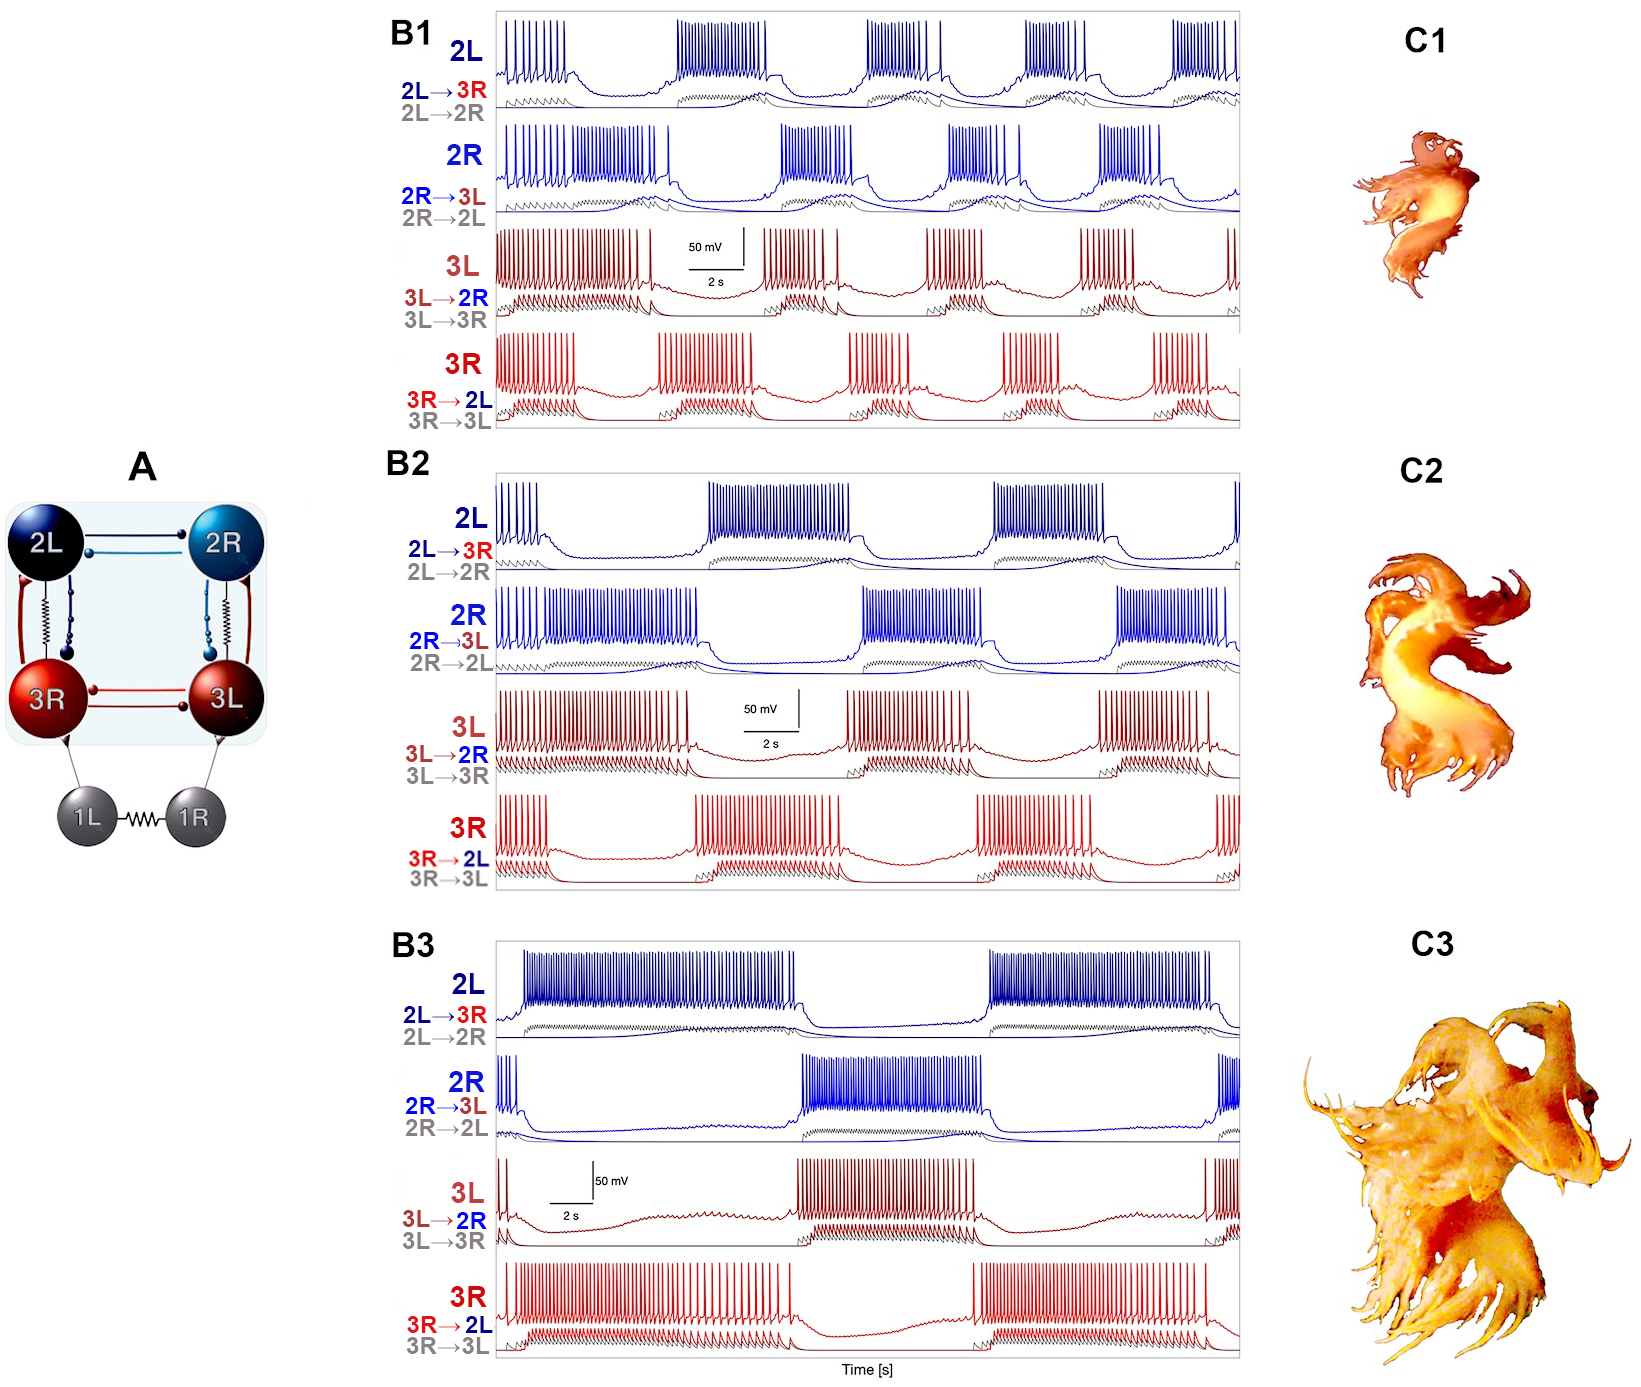
\includegraphics[width=\textwidth]{fig6.jpg}
\caption{{\bf Circuit architecture and burst frequency adaptability in the \textit{Dendronotus iris} swim CPG.}
The four-cell circuit assembles excitatory--inhibitory loops together with two contralateral half-center oscillators into a network that reliably produces left--right alternating bursts.
(A) Schematic of the canonical swim CPG circuitry composed of the four core interneurons---Si2L/R and Si3L/R---organized into two bilaterally symmetric E/I modules.
(B1--B3) Representative model traces showing voltage waveforms at three different burst frequencies, demonstrating the range of rhythmic output the network can produce.
(C1--C3) Conceptual illustration of how burst frequency modulation could accommodate variation in body size.}
\label{fig:summary}
\end{figure}

\newpage
\section*{SUPPLEMENTAL FIGURE LEGENDS}

%%% Figure S1: Additional perturbations (figS1.jpg)
\begin{figure}[htbp]
\centering
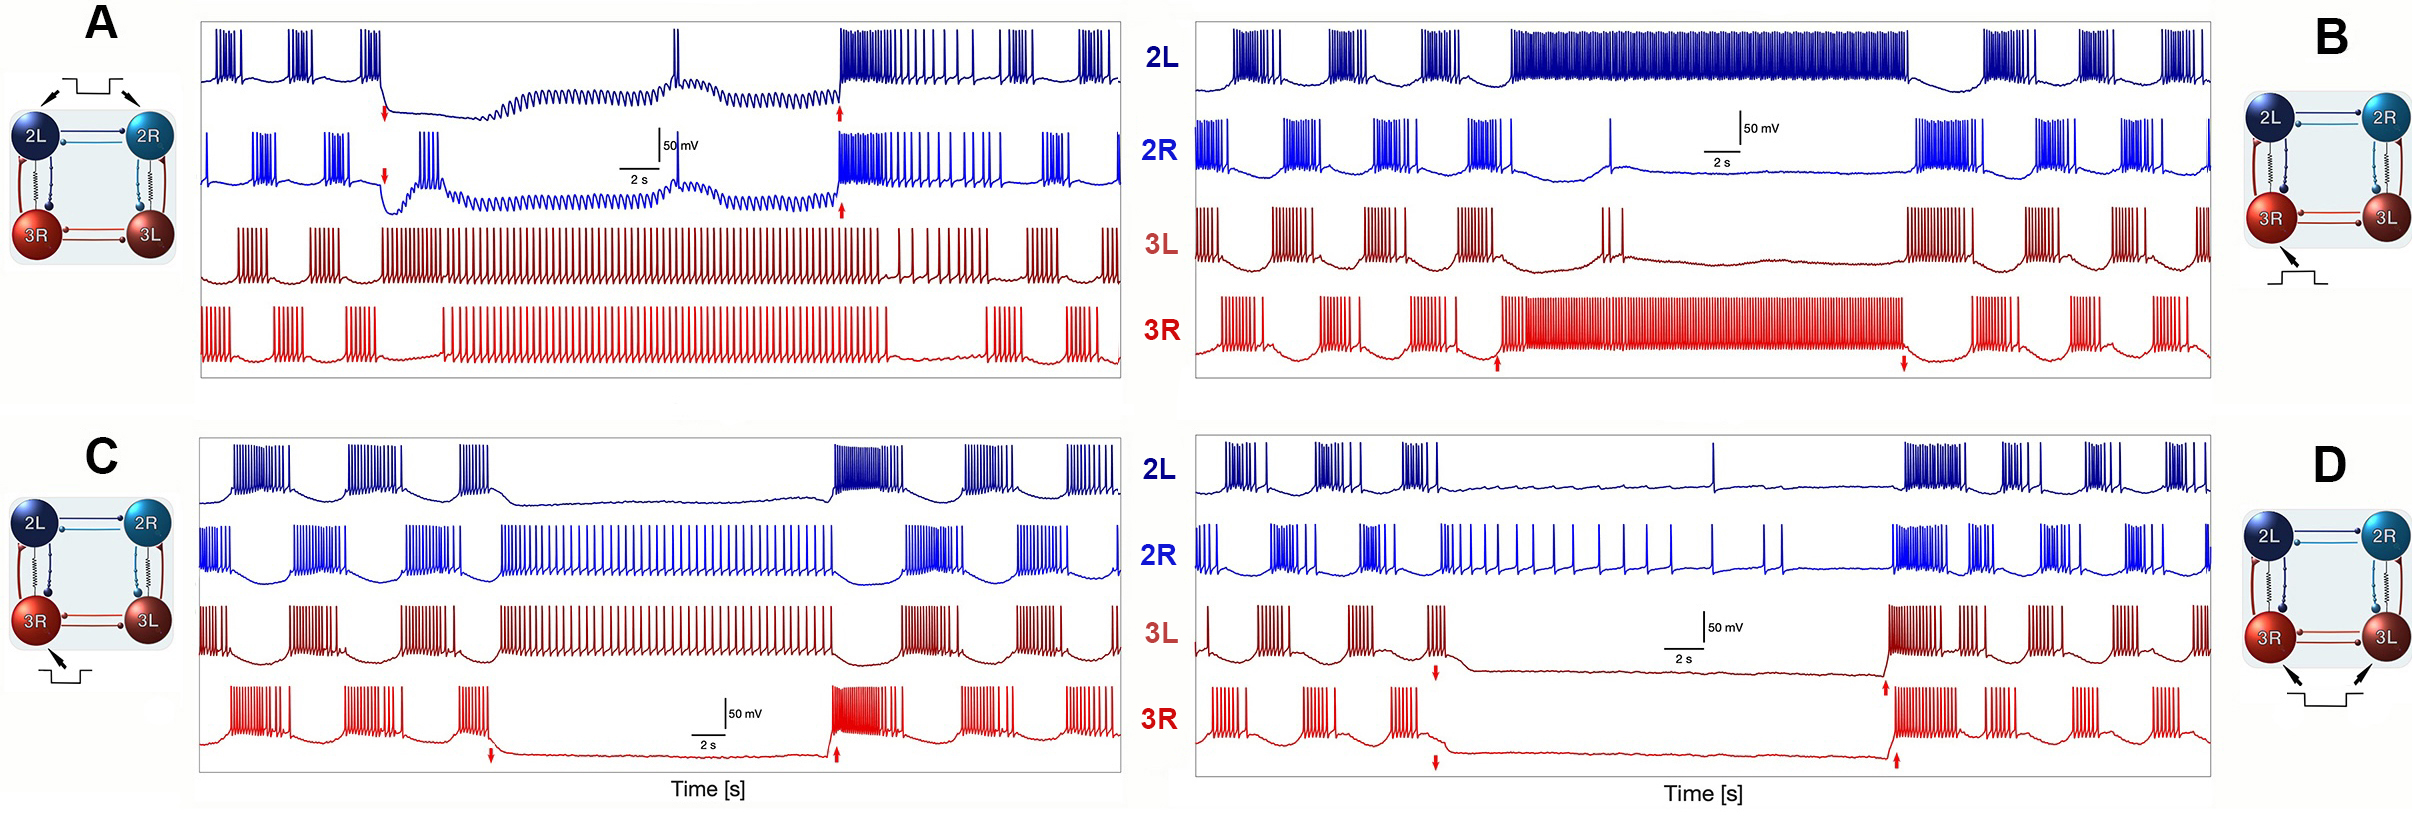
\includegraphics[width=\textwidth]{figS1.jpg}
\caption{{\bf Additional targeted perturbation experiments.}
Model responses to perturbations corresponding to Figs.~5C and E--G of Sakurai \& Katz (2016).
(A) Bilateral hyperpolarization of both Si2 neurons; the network recovers but restoration takes longer than unilateral cases.
(B) Positive current pulse to Si3R forces sustained high-frequency spiking; circuit rapidly returns to antiphase rhythm upon pulse termination.
(C) Hyperpolarizing Si3R silences it and its electrical partner Si2L.
(D) Bilateral hyperpolarization of both Si3 neurons completely abolishes network activity; rapid restoration upon pulse removal.}
\label{fig:supp_perturbations}
\end{figure}

%%% Figure S2: Symmetric perturbations (figS2.jpg)
\begin{figure}[htbp]
\centering
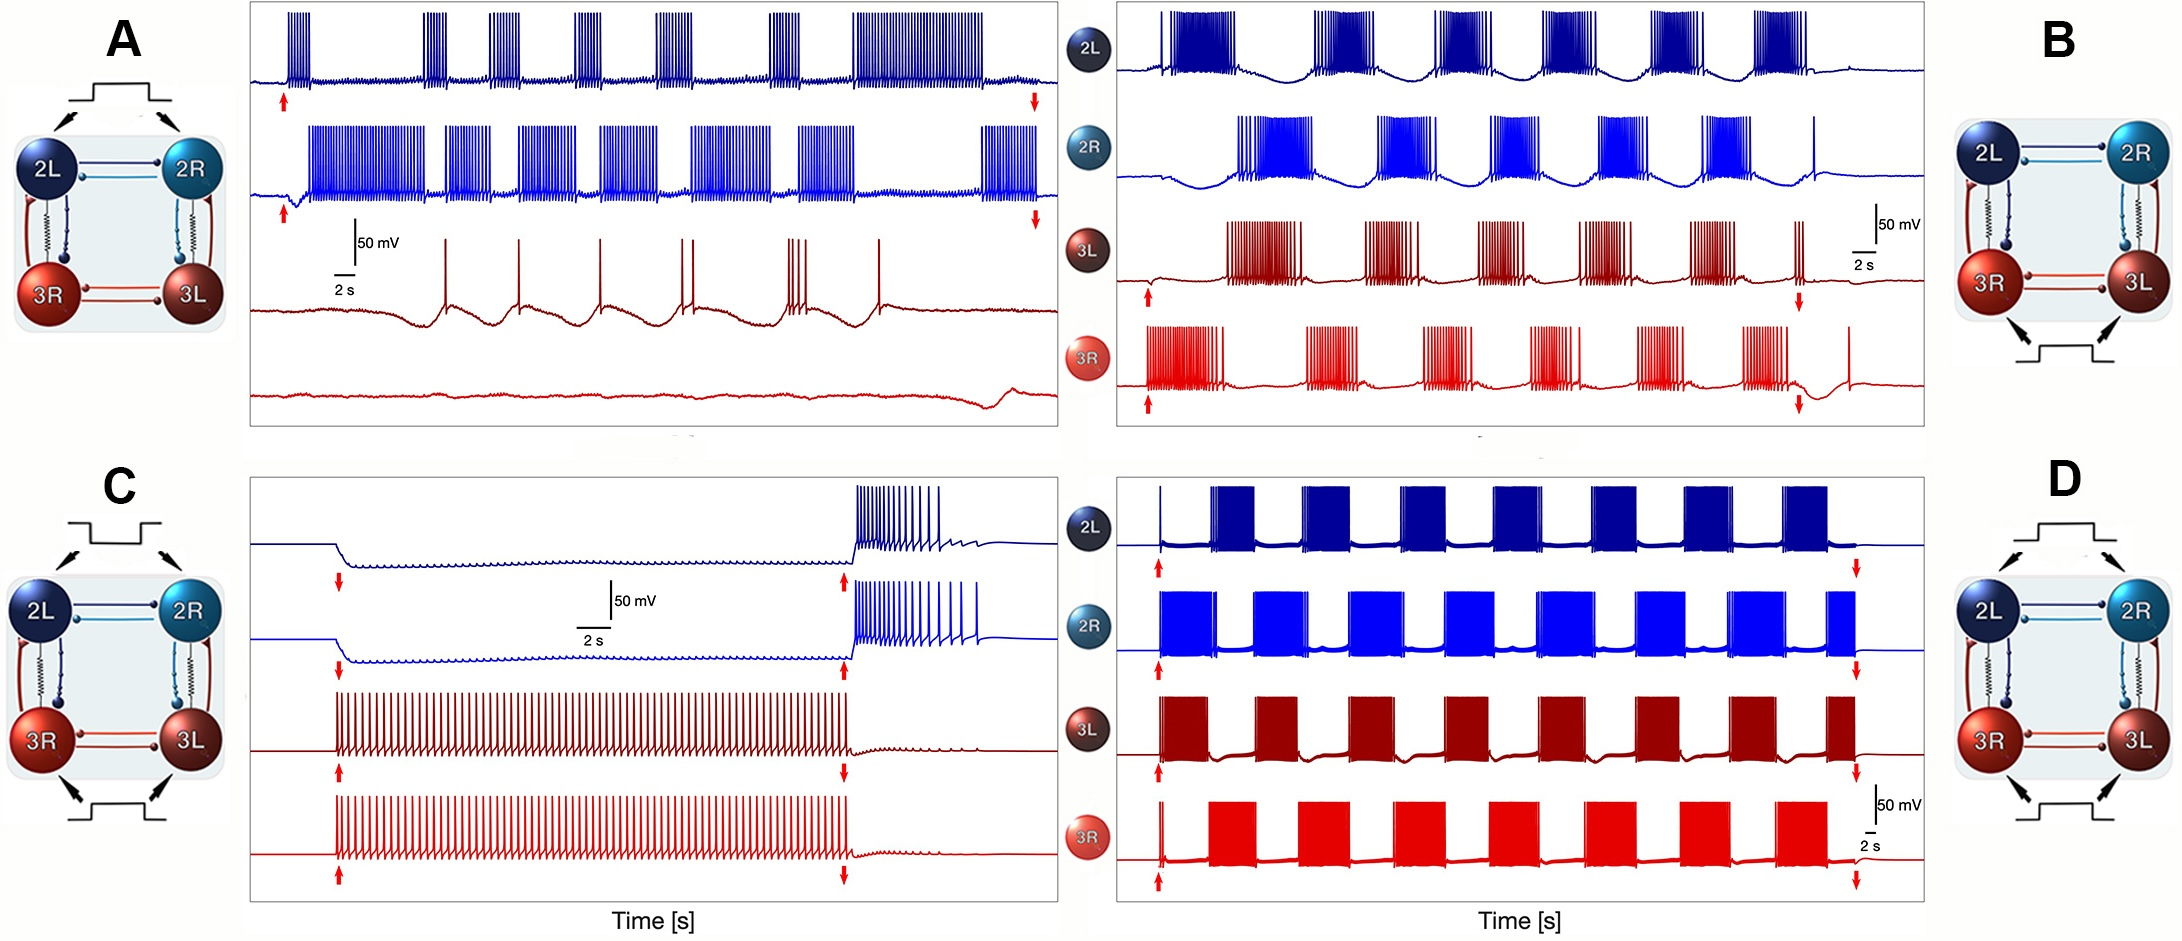
\includegraphics[width=\textwidth]{figS2.jpg}
\caption{{\bf Symmetric perturbation experiments.}
Model responses to bilateral depolarization corresponding to Fig.~7 of Sakurai \& Katz (2016).
(A--B) Bilateral depolarization of both Si2 neurons: simultaneous positive current injection into Si2L and Si2R produces coordinated high-frequency activity.
(C--D) Bilateral depolarization of both Si3 neurons: simultaneous positive current injection into Si3L and Si3R produces sustained network excitation.}
\label{fig:supp_symmetric}
\end{figure}
